\section{PROCEDIMIENTO} 

\begin{itemize}
\subsection{Parte 1: Iniciando Docker:}
	\item Abrir el menu inicio y buscar la aplicación Docker for Windows.
                    \begin{figure}[H]
		\begin{center}
		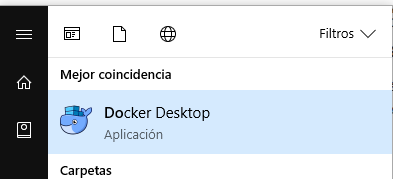
\includegraphics[width=7cm]{./Imagenes/25}
		\end{center}
		\end{figure}
	\item Una vez iniciado se podrá visualizar el icono de Docker en el área de notificación.
   \begin{figure}[H]
		\begin{center}
		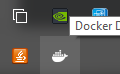
\includegraphics[width=7cm]{./Imagenes/26}
		\end{center}
		\end{figure}
          \item Asimismo se podrá visualizar la ventana de bienvenida.
          \item Ingresar sus credenciales creadas en Docker Hub para iniciar sesión en el aplicativo..
   \begin{figure}[H]
		\begin{center}
		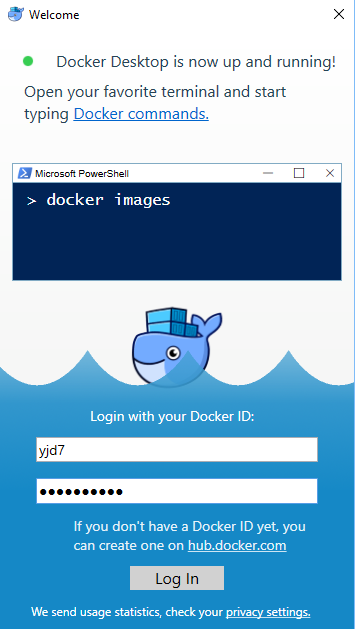
\includegraphics[width=7cm]{./Imagenes/1}
		\end{center}
		\end{figure} 
          \item Ubicar la aplicación PowerShell, ejecutarla como Administrador. En la ventana de comandos de PowerShell escribir lo siguiente: "docker versión"
                       \begin{figure}[H]
		\begin{center}
		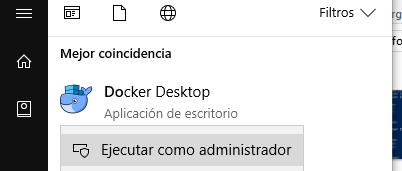
\includegraphics[width=7cm]{./Imagenes/28}
		\end{center}
		\end{figure}   

                      \begin{figure}[H]
		\begin{center}
		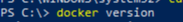
\includegraphics[width=7cm]{./Imagenes/27}
		\end{center}
		\end{figure}   
         \item Verificar que el resultado sea el siguiente.
                     \begin{figure}[H]
		\begin{center}
		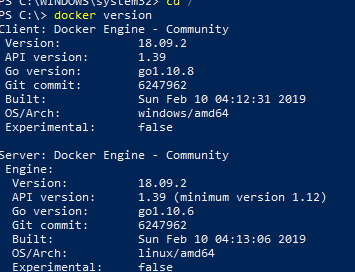
\includegraphics[width=7cm]{./Imagenes/2}
		\end{center}
		\end{figure}   
\subsection{Parte 2: Creando un contenedor con Microsoft SQL Server para Linux}
	\item En la ventana de PowerShell, escribir el siguiente comando:"docker search mssql      
	\item El resultado deberá ser algo similar a lo siguiente.
                     \begin{figure}[H]
		\begin{center}
		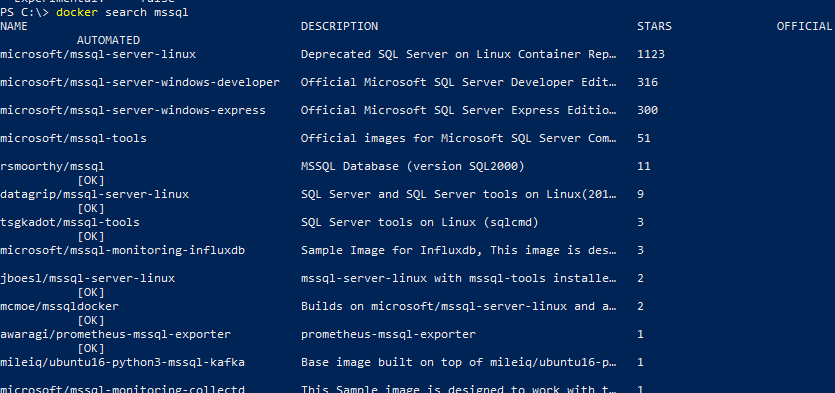
\includegraphics[width=15cm]{./Imagenes/3}
		\end{center}
		\end{figure}   
	\item Ahora ejecutar el comando:"docker pull microsoft/mssql-server-linux"
	\item Lo cual descargará la imagen del contenedor de Microsoft SQL Server en un servidor Linux
                     \begin{figure}[H]
		\begin{center}
		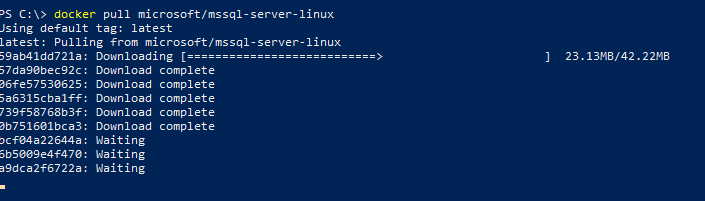
\includegraphics[width=15cm]{./Imagenes/4}
		\end{center}
		\end{figure}   
          \item Proceder a verificar la imagen con el siguiente comando:" docker images"
	\item Lo cual deberá visualizar lo siguiente:
                     \begin{figure}[H]
		\begin{center}
		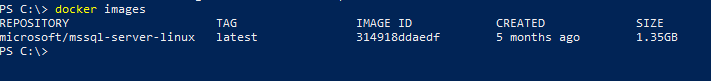
\includegraphics[width=15cm]{./Imagenes/5}
		\end{center}
		\end{figure}   
	\item Seguidamente ejecutar el comando:
                      \begin{figure}[H]
		\begin{center}
		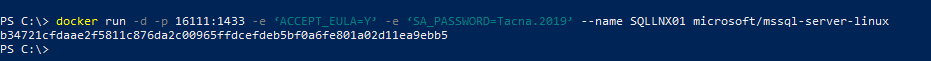
\includegraphics[width=15cm]{./Imagenes/6}
		\end{center}
		\end{figure}   
	\item Como respuesta se visualizará un ID que corresponde al contenedor:
                     \begin{figure}[H]
		\begin{center}
		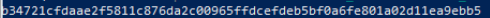
\includegraphics[width=15cm]{./Imagenes/31}
		\end{center}
		\end{figure}   
           \item Verificar que el contenedor se este ejecutando correctamente mediante el comando:" docker ps"       
	\item Si se visualiza un cuadro de dialogo de permisos relacionados al firewall Windows, Aceptarlo para realizar la conexión.El resultado será similar al siguiente:
                     \begin{figure}[H]
		\begin{center}
		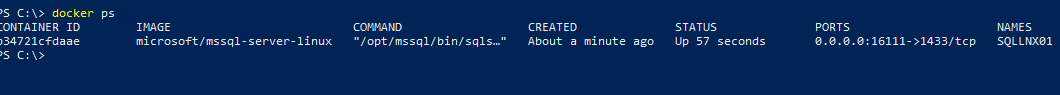
\includegraphics[width=15cm]{./Imagenes/7}
		\end{center}
		\end{figure}   
	\item . Esperar unos segundos e iniciar la aplicación Microsoft SQL Server Management Studio, y conectar con los
siguientes datos:
                      \begin{figure}[H]
		\begin{center}
		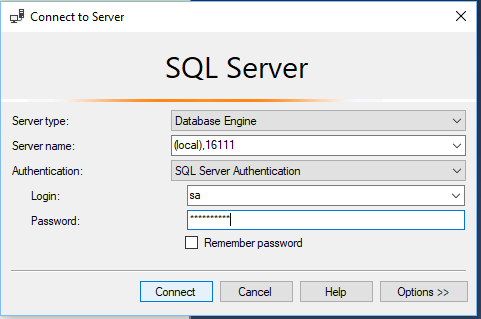
\includegraphics[width=15cm]{./Imagenes/8}
		\end{center}
		\end{figure}   
	\item Iniciar una nueva consulta, escribir y ejecutar lo siguiente:
                     \begin{figure}[H]
		\begin{center}
		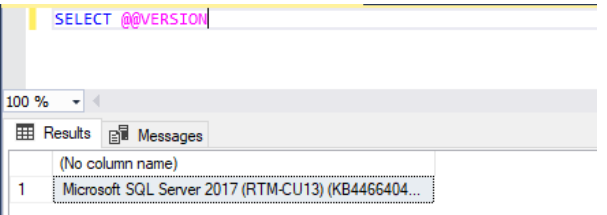
\includegraphics[width=15cm]{./Imagenes/32}
		\end{center}
		\end{figure}   
          \item Deberá retornar algo similar a lo siguiente:
                     \begin{figure}[H]
		\begin{center}
		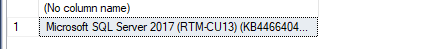
\includegraphics[width=15cm]{./Imagenes/9}
		\end{center}
		\end{figure}   
	\item Cerrar la aplicación Microsoft SQL Server Management Studio.
	\item En PowerShell ejecutar el siguiente comando:" docker rm -f SQLLNX01"
                     \begin{figure}[H]
		\begin{center}
		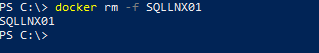
\includegraphics[width=15cm]{./Imagenes/10}
		\end{center}
		\end{figure}   
	\item Verificar la eliminación del contenedor con ejecutando: docker ps
                    \begin{figure}[H]
		\begin{center}
		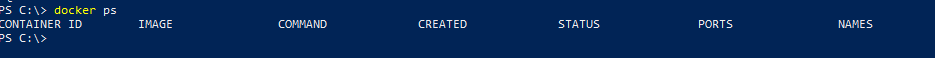
\includegraphics[width=15cm]{./Imagenes/11}
		\end{center}
		\end{figure}   
\subsection{Parte 3: Adicionando persistencia}
	\item En PowerShell ejecutar el siguiente comando.
                     \begin{figure}[H]
		\begin{center}
		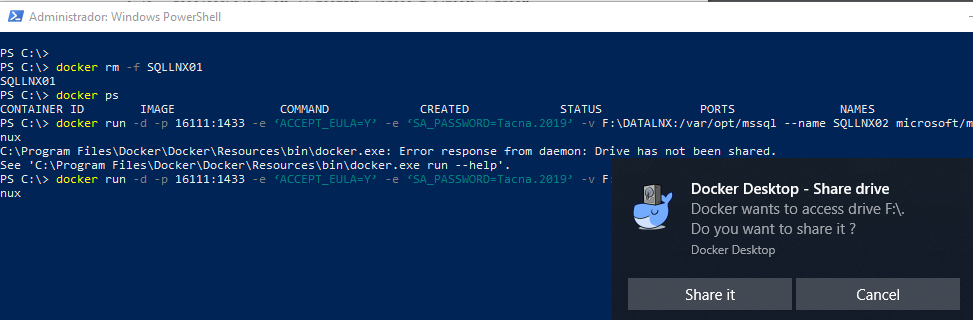
\includegraphics[width=15cm]{./Imagenes/12}
		\end{center}
		\end{figure}   
          \item luego visualizara la siguiente ventana  ingresamos las credenciales.
                     \begin{figure}[H]
		\begin{center}
		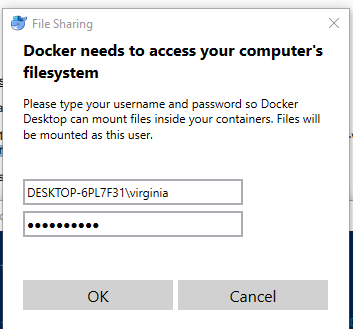
\includegraphics[width=15cm]{./Imagenes/13}
		\end{center}
		\end{figure}   
	\item Como respuesta se visualizará un ID que corresponde al contenedor:
                     \begin{figure}[H]
		\begin{center}
		
\includegraphics[width=15cm]{./Imagenes/14}
		\end{center}
		\end{figure}   
	\item Verificar que el contenedor se este ejecutando correctamente mediante el comando:
                     \begin{figure}[H]
		\begin{center}
		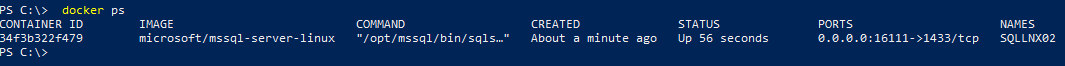
\includegraphics[width=15cm]{./Imagenes/15}
		\end{center}
		\end{figure}   
           \item Esperar unos segundos e iniciar la aplicación Microsoft SQL Server Management Studio, y conectar con los siguientes datos:
                     \begin{figure}[H]
		\begin{center}
		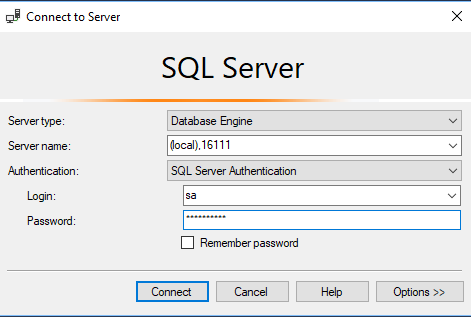
\includegraphics[width=15cm]{./Imagenes/33}
		\end{center}
		\end{figure}   
	\item Generar una base de datos de prueba en la aplicación Microsoft SQL Server Management Studio, según la siguiente imagen mediante el siguiente script:
                     \begin{figure}[H]
		\begin{center}
		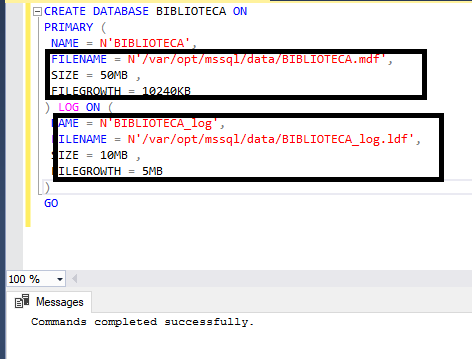
\includegraphics[width=15cm]{./Imagenes/18}
		\end{center}
		\end{figure}   
           \item Verificar el contenido la carpeta DATALNX
                     \begin{figure}[H]
		\begin{center}
		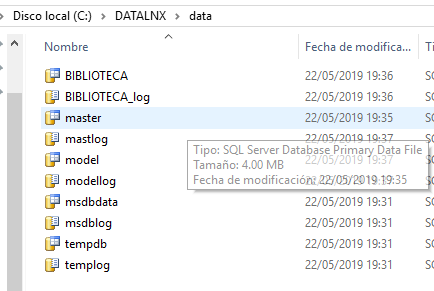
\includegraphics[width=15cm]{./Imagenes/19}
		\end{center}
		\end{figure}   
           \item En PowerShell ejecutar el siguiente comando:"docker rm -f SQLLNX02"
                      \begin{figure}[H]
		\begin{center}
		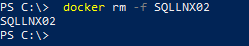
\includegraphics[width=15cm]{./Imagenes/20}
		\end{center}
		\end{figure}   
	\item Verificar la eliminación del contenedor con ejecutando:"docker ps"
                    \begin{figure}[H]
		\begin{center}
		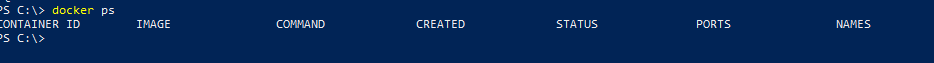
\includegraphics[width=15cm]{./Imagenes/21}
		\end{center}
		\end{figure}   
\item antes se debe compartir o elnazar la carpeta  con Docker
                    \begin{figure}[H]
		\begin{center}
		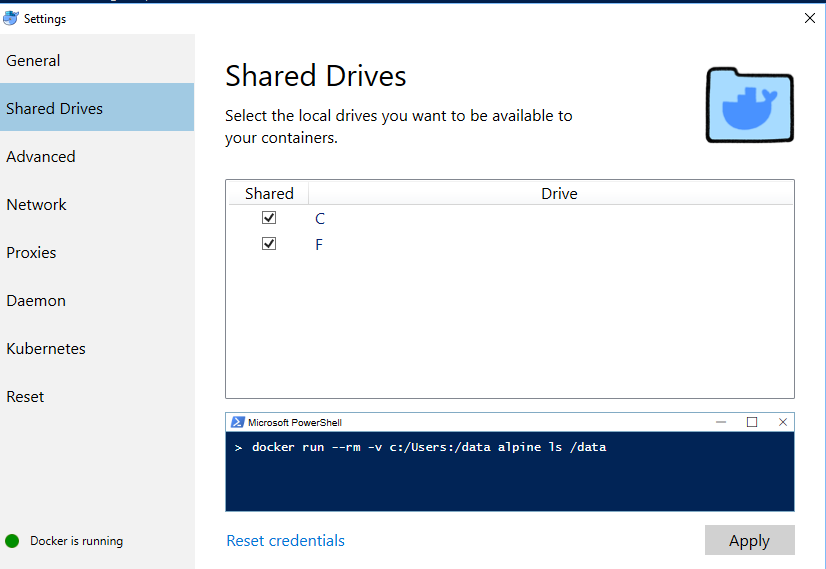
\includegraphics[width=15cm]{./Imagenes/16}
		\end{center}
		\end{figure}   
\subsection{Parte 4: Creando un contenedor con Microsoft SQL Server para Windows}
	\item En el icono de Docker en el área de notificación, hacer click con el botón derecho y utilizar la opción Switch to Windows Containers. Esperar a que Docker se reinicie.
                      \begin{figure}[H]
		\begin{center}
		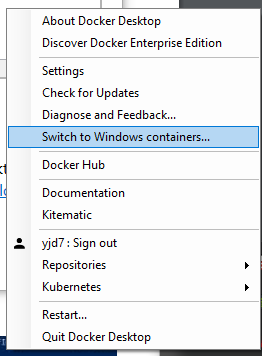
\includegraphics[width=10cm]{./Imagenes/22}
		\end{center}
		\end{figure}   
                      \begin{figure}[H]
		\begin{center}
		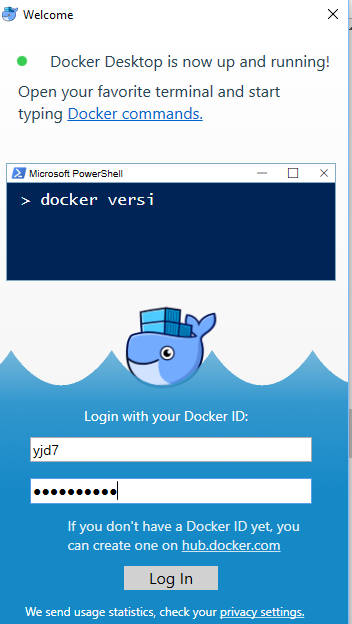
\includegraphics[width=10cm]{./Imagenes/23}
		\end{center}
		\end{figure}   
	\item En la ventana de PowerShell, escribir el siguiente comando:"docker search mssql"           
                       \begin{figure}[H]
		\begin{center}
		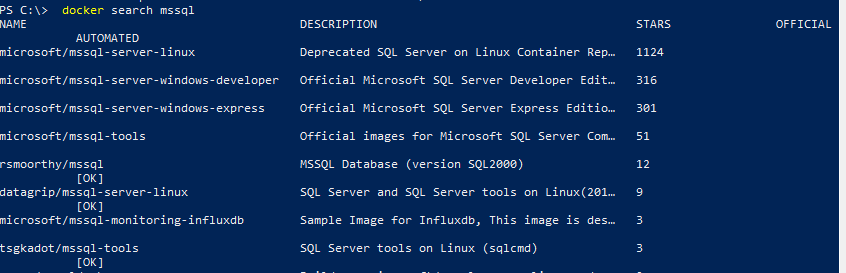
\includegraphics[width=15cm]{./Imagenes/24}
		\end{center}
		\end{figure}   
          \item Ejecutar el siguiente comando; lo cual descargará la imagen del contenedor de Microsoft SQL Server en un servidor Linux.
		\begin{figure}[H]
		\begin{center}
		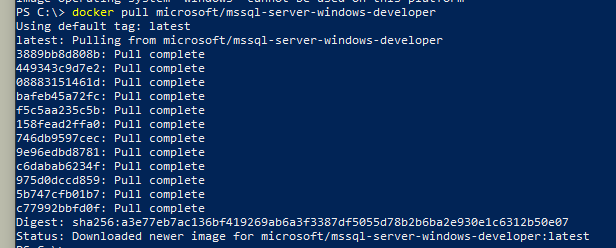
\includegraphics[width=15cm]{./Imagenes/c1}
		\end{center}
		\end{figure}  
         \item Proceder a verificar la imagen con el siguiente comando:
		\begin{figure}[H]
		\begin{center}
		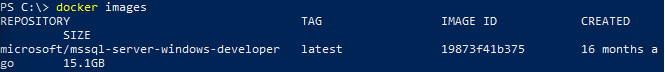
\includegraphics[width=15cm]{./Imagenes/c2}
		\end{center}
		\end{figure}  
          \item Seguidamente ejecutar el comando; como respuesta se visualizará un ID que corresponde al contenedor
		\begin{figure}[H]
		\begin{center}
		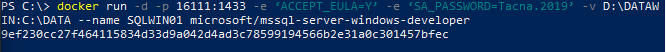
\includegraphics[width=15cm]{./Imagenes/c3}
		\end{center}
		\end{figure}  
          \item Repetir el paso 10 y verificar que el contenedor este ejecutándose
		\begin{figure}[H]
		\begin{center}
		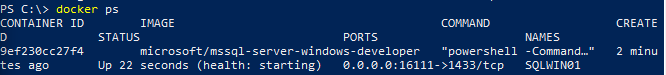
\includegraphics[width=15cm]{./Imagenes/c4}
		\end{center}
		\end{figure}  
          \item Repetir el paso 11 y conectar al servidor
		\begin{figure}[H]
		\begin{center}
		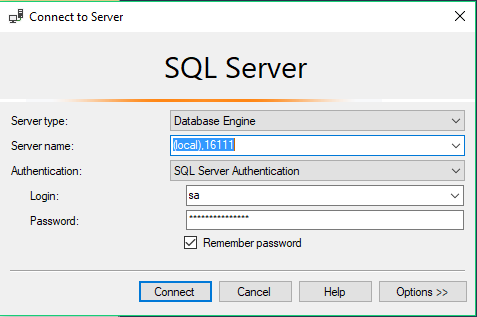
\includegraphics[width=15cm]{./Imagenes/c5}
		\end{center}
		\end{figure}  
         \item Iniciar una nueva consulta, escribir y ejecutar lo siguiente:
		\begin{figure}[H]
		\begin{center}
		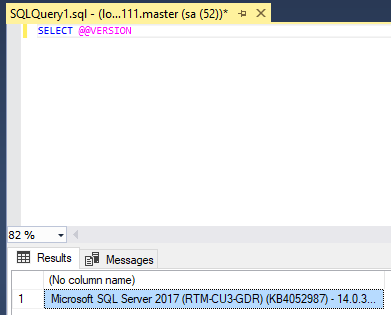
\includegraphics[width=10cm]{./Imagenes/c6}
		\end{center}
		\end{figure}  
          \item Generar una base de datos de prueba en la aplicación Microsoft SQL Server Management Studio
		\begin{figure}[H]
		\begin{center}
		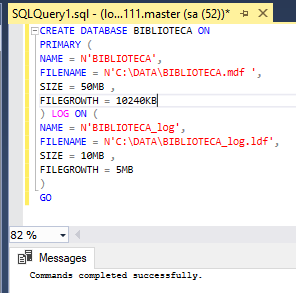
\includegraphics[width=10cm]{./Imagenes/c7}
		\end{center}
		\end{figure}  
          \item Verificar el contenido de la carpeta DATAWIN
		\begin{figure}[H]
		\begin{center}
		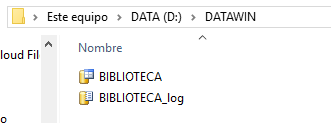
\includegraphics[width=12cm]{./Imagenes/c8}
		\end{center}
		\end{figure}  
         \item En PowerShell ejecutar el siguiente comando y verificar la eliminación del contenedor con ejecutando
		\begin{figure}[H]
		\begin{center}
		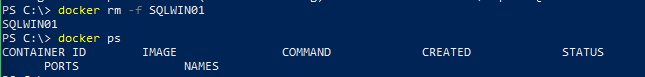
\includegraphics[width=15cm]{./Imagenes/c9}
		\end{center}
		\end{figure}  
          \item Cerrar la aplicación Microsoft SQL Server Management Studio.
       
\end{itemize}
		